\chapter{Előkészületek}

\section{Adathalmazok összeállítása}

A kitűzött céljaimhoz magyar nyelven nem állt rendelkezésre publikus adathalmaz, ezért nekem kellett ilyet összeállítanom.

\subsection{Adathalmaz háttere}

Feladatom során egy K-Monitor nevű antikorrupciós civil szervezet sajtóadatbázisának bővítését segítő rendszer fejlesztését tűztem ki célul. A szervezet évek óta gyűjt a magyar sajtóból korrupcióval és átláthatósággal kapcsolatos cikkeket az adatbázisba. Az eredeti cikkre mutató hivatkozás mellett a következő metaadatok is feljegyzésre kerülnek: a cikk címe, bevezetője (lead) és a cikkben előforduló releváns személyek, intézmények, helyszínek és egyéb kulcsszavak.

A sajtóadatbázist a K-Monitor tagjai valamint önkéntesei frissítik új cikkekkel, módszertanért lásd: \ref{appendix:kmonitor-methodology}.

Az adatbázis bővítésének asszisztálása mellett azt is kitűztem célul, hogy az egyes cikkekben megfogalmazott névelemek (személyek, intézmények) közti kapcsolatokat kinyerjem. Az ötletet a K-Monitor által működtetett Háló \cite{ahalo} adta, ami egy ilyen típusú kapcsolatokat gráf formában megjelenítő weboldal.

\subsection{Adat beszerzése}

Az adathalmazhoz 2023 januárjában adatbányászattal szereztem metaadatokat. Így jutottam hozzá 36 178 db mintához.

Emellett szükségem volt magukra a cikkek szövegére is. Ehhez elsősorban egy CommonCrawl nevű archiváló rendszerre támaszkodtam. Ami ott nem volt megtalálható azt a webről gyűjtöttem (HTTP GET lekérdezés az adott URL-re) vagy Wayback Machineről szereztem be.

\subsection{Adat tisztítás}

A különféle módon letöltött HTML dokumentumokból newspaper3k \cite{newspaper3k} Python könyvtárral nyertem ki a cikkekből lényeges részeket (cím, lead, törzs, kulcsszavak). Ez az eszköz statisztikai alapú nyelvi modelleket használ arra, hogy a természetes nyelvű szövegrészeket elválassza a felhasználói felület címkéitől. A megoldás nem volt tökéletes, ezért más módszereket is kellett alkalmaznom a felesleges szövegrészek kiszűrésére.

Az egyik probléma az volt, hogy a hírek törzsébe belekeveredtek hirdetések illetve egyéb - a tartalomhoz nem kapcsolódó - szövegrészletek. Erre a megoldásom az volt, hogy bekezdésekre bontottam a cikkeket és a cikkek között ötnél többször szó szerint előforduló bekezdéseket eltávolítottam. Ezen felül töröltem a gyanúsan rövid vagy hibás kódolású újságcikkeket is. Az így képzett adathalmaz 31 641 rekordot tartalmaz.

\subsection{Dokumentum klasszifikáció}

Mivel célom volt egy bináris klasszifikáció aszerint, hogy a cikket számunkra érdekes témában írták-e, az adathalmazba kellettek nem korrupcióról vagy átláthatóságról szóló cikkek is. Azonban ehhez nem rendelkeztem adattal, ezért nekem kellett ilyen mintákat gyűjtenem.

Elsőként kiválasztottam 36 012 db cikket manuális annotálásra, ezeket előannotáltam egy korábban tanított klasszifikációs modellel. Kiválasztottam 20 000 mintát, amit előannotálás során a modell leginkább negatívnak ítélt és ezeket negatívként beemeltem a korpuszba. Ezzel az volt a célom hogy manuálisan kevesebbet kelljen annotálnom, a művelet ára az volt, hogy hamis negatívok is bekerülhettek az adathalmazba.

A tanító- és validációs halmaz számára manuálisan annotáltam (a leginkább pozitívnak ítélt) 6 000 cikket és a teszthalmazhoz külön 2 000-et (szűrés után 1 921 db negatív minta). A teszthalmaz negatív felét csak ezek a manuálisan annotált minták adták.

Végezetül a pozitív példákkal együtt egy 55 867 rekordot tartalmazó adathalmaz keletkezett.

\subsection{Névelem klasszifikáció}

Habár a korábban részletezett adathalmaz tartalmazta a releváns személyek listáját, negatív minták nem voltak benne. Ezért elsőként futtattam egy entitásfelismerést a cikkeken HuSpaCy-vel \cite{huspacy}, így hozzájutottam a cikkben szereplő összes személyhez. Innentől pedig már a két halmaz különbsége adta a negatív mintákat.

Összesen 64 000 mintát sikerült így gyűjtenem, melyből 23 000 pozitív és 41 000 negatív.

\subsection{Kulcsszó "generálás"}

A kulcsszavak megállapításához minden szükséges adathoz hozzájutottam az adatbányászattal, ezzel további feladatom nem volt.

\subsection{Reláció kinyerés}

Az egyes névelemek közti relációkkal kapcsolatban eredetileg semmilyen adattal nem rendelkeztem a nyers szövegeken kívül, ezért itt szintetikus adathalmaz összeállítása mellett döntöttem. Ez abból állt, hogy a feladatot megoldattam egy polcról levehető nagy nyelvi modellel és a megoldásokra építve egy lokális nagy nyelvi modellt tanítottam. Ezen a ponton felmerülhet a kérdés, hogy miért nem használtam egyszerűen az eredeti modellt? A válasz az, hogy sok felhasználás esetén egy lokális modell praktikusabb, mert nagyobb kontrollt kapunk a működése felett. Emellett még kevesebb erőforrást is igényel, tehát gazdaságosabb.

Elsőként felbontottam bekezdésekre az újságcikkeket és előszűrtem, csak azokat megtartva, amik tartalmaznak legalább három entitást.

\begin{figure}[H]
	\centering
	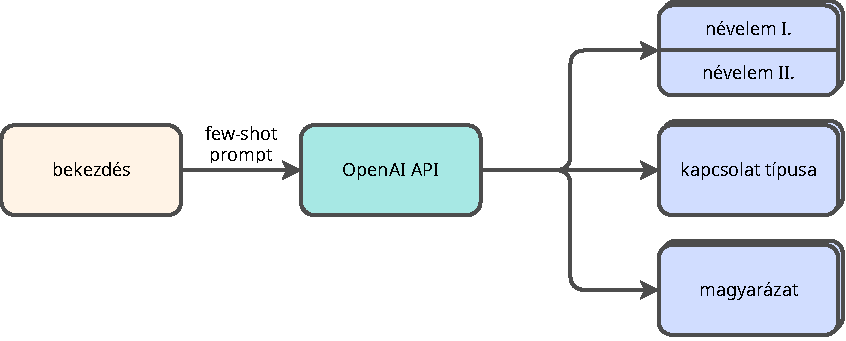
\includegraphics[width=1\textwidth]{figures/re-dataset.pdf}
	\caption{Relációkinyerési adathalmaz készítése OpenAI API segítségével}
\end{figure}

Az adathalmaz generálásához az OpenAI API-on keresztül elérhető GPT-4 turbo (gpt-4-1106-preview) és GPT-3.5 modelleket használtam. Few-shot módszert használtam a promptoláshoz. Az elvárt információ a két entitás megnevezése és a kapcsolat típusának megnevezése volt, de még egy magyarázatot is kértem a modelltől, ami egy rövid bekezdés volt.

\begin{figure}[H]
	\centering
\begin{tabular}{rrrr}
	& train & validation & test \\
	GPT-3.5 & 500 & 50 & 50 \\
	GPT-4-turbo & 600 & 60 & 60 \\
\end{tabular}
\caption{relációkinyerési adathalmaz eloszlása}
\end{figure}

\section{Kísérletek elemzése}

\subsection{Tanítási környezet}

Minden finomhangolási kísérletet egy Nvidia RTX 3060 (12GB) videokártyán végeztem. A kísérletezés átláthatóbbá tételéhez axolotl szoftvert használtam, ami lehetővé teszi, hogy egy konfigurációs fájl kitöltésével finomhangoljunk modelleket.

\subsection{Klasszifikációs módszerek összehasonlítása}

Klasszifikációs feladatra két mély-tanuláson alapuló módszert vizsgáltam meg: BERT és GPT modellek finomhangolását. A két megoldás lényegében abban különbözik, hogy míg a BERT kifejezetten támogat klasszifikációs feladatokat, addig a GPT kizárólag szöveggenerálásra képes. Viszont a klasszifikáció visszavezethető szöveggenerálási problémára, így kihasználhatjuk a GPT modellek nagyobb paraméterszámát pontosabb eredmények elérésére.

Ami viszont egy hátránya a GPT modelleknek, hogy a nagyobb paraméterszám miatt több számítási kapacitással jár a használatuk.

\begin{figure}[H]
	\centering
	\begin{tabular}{rrrr}
		modell & precision & recall  & accuracy \\
		PULI-GPT-3SX & 0.776 & 0.878 & 0.966  \\
		llama 7B & 0.860 & 0.810 & \textbf{0.971} 	\\
		huBERT & 0.739 & 0.950 & 0.963 \\
	\end{tabular}
	\caption{klasszifikációs modellek kiértékelése}
\end{figure}

\begin{figure}[H]
	\centering
	\begin{tabular}{rrrr}
		modell & gpu* inference & cpu** inference \\
		PULI-GPT-3SX & 1.90 it/s & 0.03878 it/s \\
		huBERT & 126.85 it/s & 7.10 it/s \\
	\end{tabular}
	\caption{klasszifikációs modellek teljesítménye}{
		* Nvidia 3060 12gb
		** Ampere A1 (Oracle cloud)}
\end{figure}

\subsection{Névelem klasszifikáció kiértékelése}

Névelem klasszifikációra az adathalmaz sajátosságai miatt túlságosan komplex feladat lett volna BERT modellt tanítani, ezért itt kizárólag GPT-t használtam. Ezt úgy vezettem vissza szöveggenerálási feladatra, hogy a prompt elején átadtam a HuSpaCy által felismert entitások listáját és utána a cikk szövegét.

\subsection{Reláció kinyerés}

Relációkinyeréshez az OpenAI modellek működésének reprodukálását tűztem ki célul, ezért itt adta magát egy GPT modell finomhangolása. Az viszont már nem volt teljesen egyértelmű, hogy melyik alap modell a legalkalmasabb. Kifejezetten magyar nyelvre tanított GPT modellek közül a PULI-GPT-3SX jöhet szóba, de számos többnyelvű modell jelent meg azóta fejlettebb architektúrával. Sajnos szerzői jogi okokból a modellek megosztói ellenérdekeltek a pontos tanítási adat megosztásában. Így gyakran nem tudni mennyi magyar nyelvű adatot látott egy GPT. Egy ilyen többnyelvű modell a Mistral 7B, ami a llama architektúrára épül és azt még számos új módszer beépítésével tökéletesíti. Azért, hogy össze tudjam hasonlítani a Mistral 7B-t és a modelleket, kiértékeltem mindkettőt két magyar nyelvű benchmarkon.

\begin{figure}[H]
	\centering
	\begin{tabular}{rrrr}
		modell & hucola F1 & husst F1 \\ \hline
		PULI-GPTrio & 0.523 & 0.541 \\
		PULI-GPT-3SX & 0.366 & 0.625 \\
		Mistral-7B & \textbf{0.872} & \textbf{0.636} \\
%		RWKV-World-3B & 0.865 & \textbf{0.675} \\
	\end{tabular}
	\caption{GPT modellek magyar benchmarkokon few-shot (N=5)}
\end{figure}

A kiértékelés kapcsán meg kell jegyeznem, hogy a validációs (dev) halmazt használtam, mivel a teszt minták megoldása nem nyilvános.

Mivel ennél a feladatnál nem lehet az eredeti adathalmaz megoldásában megbízni, a modell kimenetét manuálisan értékeltem ki. TODO

\subsection{Kulcsszó kinyerés eredmények}

Ebben a kulcsszókinyerési feladatban nagyon sok lehetséges kulcsszó közül kell kiválasztani az adott szövegre illőket. A sok lehetséges osztály miatt itt a BERT modellt nem találtam megfelelőnek, ezért csak GPT modellt tanítottam.

Ugyanehhez a problémához a K-Monitor által egy SpreadMonitor nevű cég számára szervezett hackathon alatt is készült egy megoldás klasszikus módszerekkel. Ez a megvalósítás BoW tokenizációra épül és Random Forest-et használ klasszifikációra. Erőssége, hogy jobb eredményeket ér el, mint a GPT-t alkalmazó megoldás, viszont cserébe minden osztályhoz külön bináris klasszifikációt kell végeznie.

\begin{figure}[H]
	\centering
	\begin{tabular}{rrrr}
		kulcsszó & GPT & BoW + RandomForest \\ \hline
		önkormányzat & 0.60 & \textbf{0.66} \\
		klientúra & 0.55 & \textbf{0.68} \\
		közbeszerzés & 0.69 & \textbf{0.74} \\
		ingatlan & 0.71 & 0.71 \\
	\end{tabular}
	\caption{F1-score eredmények néhány kulcsszóhoz}
\end{figure}
